\documentclass[10pt]{article}
\usepackage{hyperref}
\usepackage[utf8]{inputenc}
\usepackage[swedish]{babel}
\usepackage[margin=2cm]{geometry}
\usepackage{calc}
\usepackage{graphicx}
\usepackage{filecontents}
\usepackage{etoolbox}
\usepackage{enumitem}
\usepackage[backend=bibtex,sorting=none,style=numeric,natbib=true]{biblatex}
\graphicspath{ {images/}}

\selectlanguage{swedish}

\usepackage{xifthen}
\usepackage{enumitem}
\usepackage{scrextend}
\newcounter{switchcase}

\newcommand{\ifequals}[3]{\ifthenelse{\equal{#1}{#2}}{\stepcounter{switchcase} #3}{}}
\newcommand{\case}[2]{#1 #2} % Dummy, so \renewcommand has something to overwrite...
\newenvironment{switch}[1]{
  %Executed at \begin{switch}
  \setcounter{switchcase}{0}
  \renewcommand{\case}{\ifequals{#1}}
}{
 % Executed at \end{switch}
\ifthenelse{\equal{\value{switchcase}}{0}}{
  \PackageError{ProjectDefinitions}{Could not find given definition}{}}{}
}

\newcommand{\definition}[1]
{
  \begin{switch}{#1}
    \case{Cachning}{\item [\textbf{#1}]
      Temporär lagning av data för snabb åtkomst.}
    \case{Instans}{\item [\textbf{#1}]
      En spelsession som startas från UI-applikationen och spelare kan gå med i för att spela spelet tillsammans.}
    \case{IoT-backend}{\item [\textbf{#1}]
      Existerande system som kan dirigera data mellan många uppkopplade enheter.}
    \case{Kontroll-applikation}{\item [\textbf{#1}]
      Applikation som körs på en mobil eller surfplatta och tar input från användare.}
    \case{Progressive Web Apps}{\item [\textbf{#1}]
      Förkortat PWA, är ett mellanting mellan en hemsida och en applikation.
      Med en PWA behöver man inte ladda ner en app, men den ger viss funktionalitet som appar har. \cite{bib-pwa}}
    \case{Resurs}{\item [\textbf{#1}]
      Media som används i spelet, t.ex. bilder och ljud.}
    \case{Sensor}{\item [\textbf{#1}]
      En sensor som sitter på kontroll-applikationen och inte är en pekskärm, t.ex. en accelerometer.}
    \case{Server-klient-modell}{\item [\textbf{#1}]
      Struktur på ett system där någon enhet tillhandahåller resurser, information eller tjänster och flera andra enheter interagerar med denna.}
    \case{Spelläge}{\item [\textbf{#1}]
      En utökning av grundspelet som definierar speciella regler och spelmekanik.}
    \case{Spelmekanik}{\item [\textbf{#1}]
      Regler och möjligheter som definierar ett spel.}
    \case{Tunn klient}{\item [\textbf{#1}]
      Specialfall av server-klient-modell där mycket få beräkningar sker på klienten.}
    \case{UI-applikation}{\item [\textbf{#1}]
      Applikationen som kör spelet och visar spelplanen.}
    \case{Use Case Map}{\item [\textbf{#1}]
      Diagram som illustrerar hur olika händelser interagerar med arkitekturen. \cite[p.~30--33]{bib-architecture-primer}}
    \case{Scrum-board}{\item [\textbf{#1}]
      En tavla med post-it lappar som innehåller aktiviteter som ska göras under
      projektet. Detta komplementeras med olika kolumner i tavlan såsom planerad, pågående,
      testning och utgåva. Dessa bestämmer i vilket stadie lapparna befinner sig i.}
    \case{Burndown-chart}{\item [\textbf{#1}]
      En graf som visar hur många timmar medlemmarna har lagt ner i förhållande till vad som krävs för att hinna med projektet.}
    \case{Acceptanstest}{\item [\textbf{#1}]
      Slutgiltiga testet som kund utför för att se att produkten lever upp till förväntningarna.}
    \case{Enhetstest}{\item [\textbf{#1}]
      Testa varje enhet så den fungerar när den är färdig.}
    \case{Integrationstest}{\item [\textbf{#1}]
      Testa att en ny enhet som läggs till i projektet fungerar som den ska tillsammans med de andra enheterna.}
    \case{Kund}{\item [\textbf{#1}]
      Cybercom Sweden.}
    \case{Regressionstest}{\item [\textbf{#1}]
      Testa ny kod enligt gamla parametrar för att säkerställa att ingen funktionalitet försvunnit.}
    \case{Systemtest}{\item [\textbf{#1}]
      Test för att säkerställa att enheten uppfyller kraven för projektet.}
    \case{Cybercom}{\item [\textbf{#1}]
      Kortare variant av Cybercom Sweden, företaget produkten utvecklas åt.}
    \case{Enkäten}{\item [\textbf{#1}]
      Den enkät som ska användas för att utvärdera användarupplevelsen, se avsnitt  3.3 Demo och enkät.}
    \case{Kvalitet}{\item [\textbf{#1}]
        I likhet med IEEE 730 definierar denna rapport kvalitet som konformitet till projektets krav. \cite{ieee730}}
    \case{Projektet}{\item [\textbf{#1}]
        Processen att framställa en produkt åt Cybercom Sweden.}
    \case{Software Quality Asssurance}{\item [\textbf{#1}]
    	Förkortat SQA, är en samling aktiviteter som bedömmer lämpligheten och inger förtroende
    	för utvecklingsmetodiken som används.}
    \case{SQA-process}{\item [\textbf{#1}]
      I likhet med IEEE 730 definieras en SQA-process som aktiviteten att samla underlag för att med säkerhet ta
      beslutet av produkten uppnår sina kvalitetskrav}
    \case{Teamet}{\item [\textbf{#1}]
      Det team av åtta studenter som tillsammans ska utföra projektet}
    \case{Trello}{\item [\textbf{#1}]
      En hemsida för att lägga till och fördela uppgifter bland flera personer, kan liknas till en whiteboard som
      postit lappar fästs på.}
    \case{Speldata}{\item [\textbf{#1}]
      Information om handlingar och status i spelet samt nödvändig teknisk data för
      att upprätthålla kommunikation.}
    \case{Realtidsmultiplayerspel}{\item [\textbf{#1}]
      Spel där flera användares handlingar har en direkt inverkan på spelets tillstånd.}
    \case{Gamemode}{\item [\textbf{#1}]
      En variant av basspelet med eventuellt andra funktioner och regler.}
    \case{Vanliga nätverksförhållanden}{\item [\textbf{#1}]
      En enhet med en stabil internetuppkoppling utan yttre störningar.}
    \case{React}{\item [\textbf{#1}]
      Javascript-bibliotek för att bygga hemsidor och mer avancerade webbsystem.\cite{bib-react}}
    \case{Deep Stream}{\item [\textbf{#1}]
    Kommunikationssystem som tillåter synkronisering av data mellan många enheter i realtid. Tillgängligt i många olika programmeringsspråk, bland annat javascript.\cite{bib-deepstream}}
    \case{Impact Map}{\item [\textbf{#1}]
    Diagram som visar inverkan av händelser under ett mjukvarusystems livstid. Kan visa på effekterna av implementation av ny funktionalitet, fel i systemet eller säkerhetsintrång.\cite[p.~91--93]{bib-architecture-primer}}
    \case{IoT, Internet of things}{\item [\textbf{#1}]
    Internet of things -- Ett begrepp som beskriver den tekniska och samhälleliga utveckling då fler och fler saker blir uppkopplade mot internet.}
    \case{Gitrepo}{\item [\textbf{#1}]
    En datastruktur för att lagra och hantera olika versioner av kod i git.}
    \case{Master-branch}{\item [\textbf{#1}]
    Standardgrenen till ett gitrepo som vanligtvis reflekterar repot i ett fungerande tillstånd.}
	\case{Kursen}{\item [\textbf{#1}]
    Den kurs som detta projekt utförs inom, det vill säga LiTHs kurs ''Kandidatprojekt i programvaruutveckling'' med kurskod TDDD96}
  \case{npm}{\item [\textbf{#1}]
  Node Package Manager -- En pakethanterare för Javascripts ekosystem}
  \case{npm-paket}{\item [\textbf{#1}]
  Ett paket med Javascript-kod som finns tillängligt i npm}


  \end{switch}
}


\tolerance=1
\emergencystretch=\maxdimen
\hyphenpenalty=10000
\hbadness=10000

% Variable för att räkna ut magnituden på en risk.
\newcounter{indexcounter}
% Macros för risker, för att strukturera upp dem.
\newcommand{\Krav}[2]{
	\stepcounter{indexcounter}
	Krav \arabic{indexcounter} & #1 & #2 \\ \hline
}
\newcommand{\History}[3]{
	\centering #1 & #2 & #3 \\ \hline
}

\addbibresource{../references.bib}

\title{Kravspecifikation}

\author{
    Joel Almqvist\\
    \texttt{joeal360@student.liu.se}
    \and
    Björn Detterfelt\\
    \texttt{bjode786@student.liu.se}
    \and
    Tim Håkansson\\
    \texttt{timha404@student.liu.se}
    \and
    David Kjellström\\
    \texttt{davkj168@student.liu.se}
    \and
    Axel Löjdquist\\
    \texttt{axelo225@student.liu.se}
    \and
    Joel Oskarsson\\
    \texttt{joeos014@student.liu.se}
    \and
    Lieth Wahid\\
    \texttt{liewa893@student.liu.se}
    \and
    Alexander Wilkens\\ 
    \texttt{alewi684@student.liu.se}
}

\date{\today \\Version 2.0}

\begin{document}

\maketitle
\pagebreak

\section*{Dokumenthistorik}

\begin{center}
    \begin{tabular}{|p{1.5cm}|p{2cm}|p{12cm}|}
    	\hline
        \textbf{Version} & \textbf{Datum} & \textbf{Förändring och kommentar} \\ \hline
        \History{1.0}{2018-02-15}{Första utkast till kund}
        \History{1.1}{2018-02-16}{Uppdaterat stavning, definitioner, formulerat om krav 3, 9, 11, 16, 22 ,23 \& 24. Tog bort krav 12, 13, 17, 19, 20 \& 21. (Kund)}
        \History{1.2}{2018-02-19}{Uppdaterat stavning, formulerat om krav 8 \& 16. (Kund)}
        \History{1.3}{2018-02-22}{Uppdaterat stavning, formulerat om krav 6, 8, 10, 13, 15, 17, 22, 23, 28 \& 32. (Kund)}
        \History{2.0}{2018-02-27}{Uppdaterat stavning och struktur. Lagt till en översiktlig bild av systemet. Formulerat om krav 17, 24, 33  \& 34. (Handledare)}
    \end{tabular}
\end{center}

\pagebreak
\tableofcontents
\pagebreak

\section{Inledning}
	I detta kapitel definieras och introduceras kontexten för projektet som ska utföras.

	\subsection{Definitioner}
		\begin{itemize}[leftmargin=5cm]
      \definition{UI-applikation}
      \definition{Kontroll-applikation}
      \definition{Sensor}
      \definition{Instans}
      \definition{Progressive Web Apps}
      \definition{Realtidsmultiplayerspel}
      \definition{Gamemode}
      \definition{Vanliga nätverksförhållanden}
		\end{itemize}	

	\subsection{Parter}
	Kunden till projektet är Cybercom Sweden. Projektet utförs av projektgruppens medlemmar.
	
	\subsection{Syfte \& mål}
	Syftet med kravspecifikationen är att förtydliga vad som förväntas vara klart vid projektets slut. Dokumentet fungerar som överenskommelse mellan kunden Cybercom Sweden och projektgruppen. Kraven specificerar vilken funktionallitet, kvalitet och design produkten ska uppfylla. Dokumentet utgör grunden för hur hela projektet ska struktureras och utformas. Kraven är framtagna efter Cybercom Swedens önskemål och formulerade för att ligga till stöd för projektgruppensarbete.
	
	\subsection{Användning}
		För att kunna använda produkten måste två olika applikationer köras på minst två olika enheter. En mobil eller surfplatta ska användas som kontroll för att styra spelet och kommer att köra kontrollapplikationen. Utöver detta ska en enhet som t.ex. en dator vara uppkopplad till en skärm. Datorn ska köra själva spelet och kommer att köra UI-applikationen. Se figur \ref{fig:overview} för en översiktlig bild av systemet. \\
\\
För att kunna använda produkten startar man UI-applikationen. Då UI-applikationen körs igång, skapas en spelinstans där en identifikationskod kommer att genereras och visas på skärmen. För att kunna ansluta sig till den spelinstansen behöver en användare starta kontrollapplikationen. Här kommer användaren få möjlighet att ange ett användarnamn, om inget användarnamn anges, slumpas ett användarnamn fram. Användaren kommer även behöva välja i en lista den spelinstans användaren vill ansluta sig till.  Efter att användaren valt spelinstans, är spelet redo att spelas.

\pagebreak

\section{Översikt av Systemet}
	Detta kapitel ger en överskådlig blick av systemet.
	
	\begin{figure}[h]
		\centering
		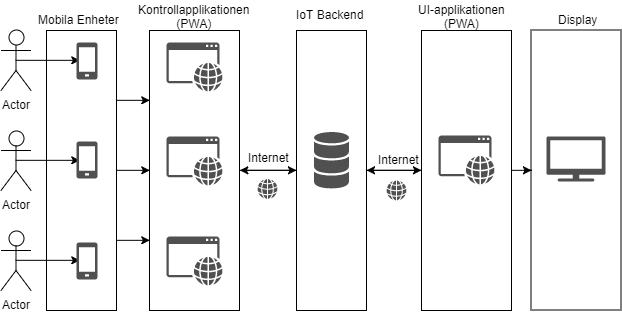
\includegraphics[scale=0.8]{overview}
		\caption{Översikt av systemet}
		\label{fig:overview}
	\end{figure}

	\subsection{Grov beskrivning av produkten}
	Produkten ska vara ett realtidsmultiplayerspel. Spelet är uppdelat i två olika applikationer, en UI-applikation och en kontrollapplikation. Det är tänkt att UI-applikationen ska agera skärm för spelet och kan liknas med en konsol för ett TV-spel. På denna del kommer själva spelet köras och vara uppkopplad till en skärm där spelet visas. En kontroller kommer vara antingen en mobil eller surfplatta och kan liknas med spelkontrollerna till konsolen. Enhetens sensorer används för att spelaren ska kunna styra spelet. Kommunikationen mellan UI-applikationen och kontrollapplikationen kommer att ske genom Cybercoms IoT-backend, se figur \ref{fig:backend}. Att kommunikationen går genom Cybercoms IoT-backend är vitalt eftersom huvudsyftet med projektet är att demonstrera Cybercoms IoT-backend.  Både kontroll- och UI-Applikationen kommer att utvecklas som PWA:s. 
	
	\begin{figure}[h]
		\centering
		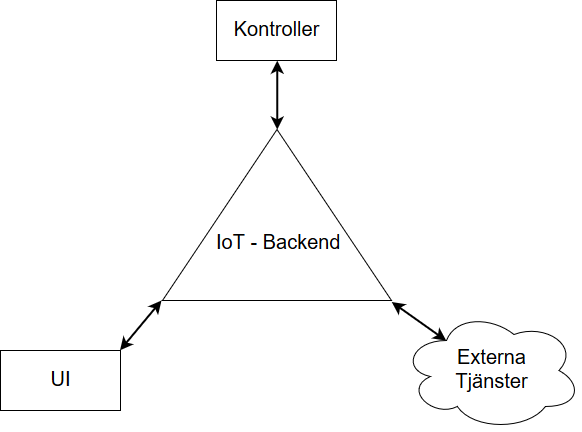
\includegraphics[scale=0.4]{backend}
		\caption{Kommunikation mellan Cybercoms IoT-backend och komponenterna i systemet}
		\label{fig:backend}
	\end{figure}
	
	
	\subsection{Beroenden av andra system}
	Produkten är beroende av Cybercoms IoT-backend då all kommunikation måste gå genom denna. Både kontroll- och UI-applikationen är beroende av en enhet som har tillgång till version 64 av Google Chrome. En enhet kan t.ex. vara en dator, surfplatta eller en mobil. Enheten måste ha en internetanslutning.

\pagebreak
\section{Krav}
	Detta avsnitt listar alla krav som sätts på produkten. Krav med prioritet 1 förväntas vara avklarade vid projektetsslut. Krav med prioritet 2 ska arbetas mot då alla krav med prioritet 1 är avklarade. Kraven är uppdelade i följande kategorier: funktionella krav och design- och kvalitetskrav. Varje krav består av ett unikt nummer, en beskrivning samt en prioritet.
	
	\subsection{Funktionella Krav}
	Detta avsnitt listar de funktionella kraven på produkten. Funktionella krav deklarerar vilka beteenden och attribut produkten förväntas ha. 

	\subsubsection*{Generella krav}
	Nedan följer generella krav för både kontroll- och UI-applikationen.\\
	
	\begin{tabular}{| p{2cm} | p{8cm} | p{2cm}|}
		\hline
		
		\textbf{Krav nr.} & \textbf{Beskrivning} &\textbf{Prioritet} \\ \hline
		\Krav{En mobil eller surfplatta ska användas som spelkontroll för spelet.}{1}
		\Krav{UI-applikationen ska endast kommunicera med \newline kontrollapplikationen via  Cybercoms IoT-backend.}{1}
		\Krav{En användare ska kunna ansluta sig till en spelinstans.}{1}
		\Krav{Flera instanser av spelet ska kunna köras samtidigt.}{1}
		\Krav{En unik slumpmässig identifikationskod ska genereras för en spelinstans.}{1}
		\Krav{Spelet ska stödja flera gamemodes.}{2}
		\Krav{En spelare ska ha möjligheten att rösta på vilket gamemode som ska spelas.}{2}
				
	\end{tabular}

	\subsubsection*{Krav kontrollapplikation}
	Nedan följer krav specifika för kontrollapplikationen.\\

	\begin{tabular}{| p{2cm} | p{8cm} | p{2cm}|}
		\hline
		
		\textbf{Krav nr.} & \textbf{Beskrivning} &\textbf{Prioritet} \\ \hline
		\Krav{Kontrollapplikationen ska ha ett grafiskt gränssnitt.}{1}
		\Krav{Spelaren ska kunna sätta ett användarnamn.}{1}
		\Krav{Om en spelare inte anger ett användarnamn, ska ett användarnamn ges till spelaren.}{1}
		\Krav{Kontrollapplikationen ska köras på en enhet som har minst version 64 av Google Chrome.}{1}
		\Krav{Kontrollapplikationen ska ansluta sig till en spelinstans genom att välja en spelinstans från en lista.}{1}
		\Krav{Kontrollapplikationen ska ha en sökruta, för att kunna söka bland de olika spelinstanserna.}{1}
		\Krav{Kontrollapplikationen ska kommunicera med Cybercoms IoT-backend.}{1}
		\Krav{Kontrollapplikationen ska kunna kalibrera en accelerometer.}{1}
		\Krav{Kontrollapplikationen ska stödja alternativa styrningsmetoder i de fall sensorer saknas.}{2}
		\Krav{Kontrollapplikationen ska stödja styrning med tangentbord och mus.}{2}

	\end{tabular}

	\pagebreak
	\subsubsection*{Krav UI-applikation}
	Nedan följer krav specifika för UI-applikationen.\\

	\begin{tabular}{| p{2cm} | p{8cm} | p{2cm}|}
		\hline
		
		\textbf{Krav nr.} & \textbf{Beskrivning} &\textbf{Prioritet} \\ \hline
		\Krav{UI-applikationen ska stödja minst fem spelare samtidigt.}{1}
		\Krav{UI-applikationen ska ha ett grafiskt gränssnitt.}{1}
		\Krav{UI-applikationen ska kunna köras på en enhet som har minst version 64 av Google Chrome.}{1}
		\Krav{UI-applikationen ska kommunicera med Cybercoms IoT-backend.}{1}
		\Krav{UI-applikationen ska visa en unik kod för sin spelinstans.}{1}
		\Krav{UI-applikationen ska arkitekturellt ha stöd för godtyckligt antal spelare. Hårdvara, prestanda och plats på skärmen begränsar.}{2}
		\Krav{UI-applikationen ska kunna visa det som andra UI-applikationer visar i realtid.}{2}
						
	\end{tabular}
	
	\subsection{Designkrav}
	Detta avsnitt listar designkraven på produkten. Designkrav specificerar hur produkten ska utformas och ställer krav på hur utvecklingsprocessen kommer gå tillväga.  \\
	
	\begin{tabular}{| p{2cm} | p{8cm} | p{2cm}|}
		\hline
		\textbf{Krav nr.} & \textbf{Beskrivning} & \textbf{Prioritet} \\ \hline
		
		\Krav{UI-applikationen ska skrivas i Javascript ES2015+.}{1}
		\Krav{Kontrollapplikationen ska skrivas i Javascript ES2015+.}{1}
		\Krav{UI-applikationen ska utvecklas som en PWA.}{1}
		\Krav{Kontrollapplikationen ska utvecklas som en PWA.}{1}
		\Krav{UI-applikationen ska licensieras under MITs open source licens.}{1}
		\Krav{Kontrollapplikationen ska licensieras under MITs open source licens.}{1}
		\Krav{Applikationsprojekten ska vara Node-baserade.}{1}
		
	\end{tabular}
\pagebreak
	\subsection{Kvalitetskrav}
	Detta avsnitt listar kvalitetskraven på produkten. Kvalitetskrav specificerar hur väl ett attribut hos produkten måste funktionera. D.v.s. vilka kvaliteter en lösning måste ha eller under vilka förhållanden lösningen måste fungera inom. Projektgruppen har valt att verifiera vissa av dessa kvalitetskrav med hjälp av en enkätundersökning. Enkäten är definerad i kvalitetsplanen. \\
	
		\begin{tabular}{|p{2cm}|p{8cm}|p{2cm}|}
		\hline
		\textbf{Krav nr.} & \textbf{Beskrivning} & \textbf{Prioritet} \\ \hline
		
		\Krav{UI-applikationen ska kunna köras i 4 timmar utan avbrott.}{1}
		\Krav{Koden ska följa en enhetlig standard\cite{bib-kvalitetsplan} för att underlätta vidareutveckling av projektet.}{1}
		\Krav{Tiden att ansluta sig till en spelsession får inte överskrida 10 sekunder under vanliga nätverksförhållanden.}{1}
        \Krav{Enkätens\cite{bib-kvalitetsplan} genomsnittliga betyg för responsivitet ska åtminstone vara 6 av 10 vid en undersökning av 20 deltagare.}{1}
		\Krav{Enkätens\cite{bib-kvalitetsplan} genomsnittliga betyg för användbarhet ska åtminstone vara 6 av 10 vid en undersökning av 20 deltagare.}{1}
		\Krav{Enkätens\cite{bib-kvalitetsplan} genomsnittliga betyg för den alternativa styrningen ska åtminstone vara 6 av 10 vid en undersökning av 20 deltagare.}{1}
		\Krav{Enkätens\cite{bib-kvalitetsplan} genomsnittliga betyg för ''lätt att förstå vad som händer'' ska åtminstone vara 6 av 10 vid en undersökning av 20 deltagare.}{1}
				
	\end{tabular}
	

\pagebreak

\printbibliography
\addcontentsline{toc}{section}{\refname}


\end{document}
